%!TEX program = xelatex
% PhD Thesis
\documentclass[letterpaper,12pt,twoside]{memoir}

% thesis metadata
\newcommand{\thesistitle}{Statistical Topology of Reticulate Evolution}
\newcommand{\thesisauthor}{Kevin Joseph Emmett}
\newcommand{\thesisyear}{2015}
\newcommand{\abstractpath}{./tex/abstract.tex}

% load thesis styling
\usepackage{thesis}

% bibliography setup
\usepackage[backend=biber,style=numeric,sorting=nyt,bibencoding=utf8]{biblatex}
\addbibresource{./thesis.bib}
\setlength{\bibitemsep}{\baselineskip} % skip line between bib entries

% document
\begin{document}

% cover pages [no numbering]
\thesistitlepage
\thesiscopyrightpage
\thesisabstract

% prefatory pages [roman numerals]
\frontmatter

\tableofcontents
\cleardoublepage

\listoffigures
\cleardoublepage

\listoftables
\cleardoublepage

\thesisacknowledgements

\thesisdedication

% main body [arabic numerals]
\mainmatter

% introduction
%!TEX root = ../thesis.tex
\chapter{Introduction}
\label{ch:introduction}

\epigraph{``I predict a new subject of statistical topology. Rather than count the
number of holes, Betti numbers, etc., one will be more interested in the
distribution of such objects on noncompact manifolds as one goes out
to infinity''}{Isadore Singer}

This thesis contains results of applying methods from topological data analysis to various problems in genomics and evolution.
It primarily details the use of persistent homology as a tool to measure the prevalence and scale of nonvertical evolutionary events, such as reassortments and recombinations.
In so doing, various techniques are developed to extract statistical information from the topological complexes that are constructed.
We rely on results from \cite{Grosz_and_Sidner_1986}.

This thesis contains results of applying methods from topological data analysis to various problems in genomics and evolution.
It primarily details the use of persistent homology as a tool to measure the prevalence and scale of nonvertical evolutionary events, such as reassortments and recombinations.
In so doing, various techniques are developed to extract statistical information from the topological complexes that are constructed.
We rely on results from \cite{Grosz_and_Sidner_1986}.

This thesis contains results of applying methods from topological data analysis to various problems in genomics and evolution.
It primarily details the use of persistent homology as a tool to measure the prevalence and scale of nonvertical evolutionary events, such as reassortments and recombinations.
In so doing, various techniques are developed to extract statistical information from the topological complexes that are constructed.
We rely on results from \cite{Grosz_and_Sidner_1986}.

This thesis contains results of applying methods from topological data analysis to various problems in genomics and evolution.
It primarily details the use of persistent homology as a tool to measure the prevalence and scale of nonvertical evolutionary events, such as reassortments and recombinations.
In so doing, various techniques are developed to extract statistical information from the topological complexes that are constructed.
We rely on results from \cite{Grosz_and_Sidner_1986}.

This thesis contains results of applying methods from topological data analysis to various problems in genomics and evolution.
It primarily details the use of persistent homology as a tool to measure the prevalence and scale of nonvertical evolutionary events, such as reassortments and recombinations.
In so doing, various techniques are developed to extract statistical information from the topological complexes that are constructed.
We rely on results from \cite{Grosz_and_Sidner_1986}.

This thesis contains results of applying methods from topological data analysis to various problems in genomics and evolution.
It primarily details the use of persistent homology as a tool to measure the prevalence and scale of nonvertical evolutionary events, such as reassortments and recombinations.
In so doing, various techniques are developed to extract statistical information from the topological complexes that are constructed.
We rely on results from \cite{Grosz_and_Sidner_1986}.

This thesis contains results of applying methods from topological data analysis to various problems in genomics and evolution.
It primarily details the use of persistent homology as a tool to measure the prevalence and scale of nonvertical evolutionary events, such as reassortments and recombinations.
In so doing, various techniques are developed to extract statistical information from the topological complexes that are constructed.
We rely on results from \cite{Grosz_and_Sidner_1986}.

This thesis contains results of applying methods from topological data analysis to various problems in genomics and evolution.
It primarily details the use of persistent homology as a tool to measure the prevalence and scale of nonvertical evolutionary events, such as reassortments and recombinations.
In so doing, various techniques are developed to extract statistical information from the topological complexes that are constructed.
We rely on results from \cite{Grosz_and_Sidner_1986}.

This thesis contains results of applying methods from topological data analysis to various problems in genomics and evolution.
It primarily details the use of persistent homology as a tool to measure the prevalence and scale of nonvertical evolutionary events, such as reassortments and recombinations.
In so doing, various techniques are developed to extract statistical information from the topological complexes that are constructed.
We rely on results from \cite{Grosz_and_Sidner_1986}.



\chapter{Theory}
\label{ch:theory}
%!TEX root = ../thesis.tex

For further information on mapper, see \cite{Singh:2007}.
For further information on persistent homology, see \cite{Zomorodian:2005a,Zomorodian:2005b}.

%% Part 1: Models
\part{Theory}
\label{part:theory}

In this section, we consider two models.

\chapter{Parametric Inference using Persistence Diagrams}
\label{ch:parametric_inference}
%!TEX root = ../thesis.tex

\section{Persistent Homology}

We summarize persistent homology from the perspective of an end-user.
For detailed background, see the reviews \cite{Carlsson:2009,Ghrist:2008} and the books \cite{Edelsbrunner:2010,Zomorodian:2005b}.
In brief, persistent homology computes topological invariants representing information about the connectivity and holes in a dataset.
A dataset, $S=(s_{1},\ldots,s_{N})$, is represented as a point cloud in a high-dimensional space (not necessarily Euclidean).
From the point cloud, a nested family of simplicial complexes, or a filtration, is constructed, parameterized by a filtration value $\epsilon$, which controls the simplices present in the complex.
The two most common ways of constructing a simplicial complex at each $\epsilon$ are the \v{C}ech complex and the Vietoris-Rips complex.
The filtration is represented as a list of simplices defined on the vertices of $S$, annotated with the $\epsilon$ at which the simplex appears.
Given a filtration, the persistence algorithm is used to compute homology groups.
The $0$-dimensional homology ($H_0$) represents a hierarchical clustering of the data.
Higher dimensional homology groups represent loops, holes, and higher dimensional voids in the data.
Each feature is annotated with an interval, representing the $\epsilon$ at which the feature appears and the $\epsilon$ at which the feature contracts in the filtration.
These filtration values are the \emph{birth} and \emph{death} times, respectively.
The topological invariants in the filtration can be concisely represented in a barcode diagram, a set of line segments ordered by filtration value on the horizontal axis (Figure \ref{fig:persistence_diagram}).
Equivalently, invariants can represented by a persistence diagram, a scatter plot with the birth time on the horizontal axis and the death time on the vertical axis .
Persistent homology is computed using Dionysus \cite{Morozov:2012}.

\begin{figure}
\begin{center}
\centerline{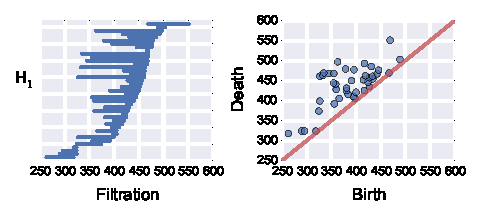
\includegraphics[width=\columnwidth]{./fig/persistence_diagram.pdf}}
\caption[Two representations of the same topological invariants computed using persistent homology]{Two representations of the same topological invariants, computed using persistent homology. Left: Barcode diagram. Right: Persistence diagram. Data was generated from a coalescent simulation with $n=100$, $\rho=72$, and $\theta=500$.}
\label{fig:persistence_diagram}
\end{center}
\end{figure}

\section{Coalescent Process}

The coalescent process is a stochastic model that generates the genealogy of individuals sampled from an evolving population \cite{Wakeley:2009}.
The genealogy is then used to simulate the genetic sequences of the sample.
This model is essential to many methods commonly used in population genetics.
Starting with a present-day sample of $n$ individuals, each individual's lineage is traced backward in time, towards a mutual common ancestor.
Two separate lineages collapse via a coalescence event, representing the sharing of an ancestor by the two lineages.
The stochastic process ends when all lineages of all sampled individuals collapse into a single common ancestor.
In this process, if the total (diploid) population size $N$ is sufficiently large, then the expected time before a coalescence event, in units of $2N$ generations, is approximately exponentially distributed:
\begin{equation}
P(T_{k}=t) \approx \binom{k}{2} e ^{-\binom{k}{2} t},
\end{equation}
where $T_k$ is the time that it takes for $k$ individual lineages to collapse into $k-1$ lineages.

After generating a genealogy, the genetic sequences of the sample can be simulated by placing mutations on the individual branches of the lineage.
The number of mutations on each branch is Poisson-distributed with mean $\theta t / 2$, where $t$ is the branch length and $\theta$ is the population-scaled mutation rate.
In this model, the average \emph{genetic distance} between any two sampled individuals, defined by the number of mutations separating them, is $\theta$.

The coalescent with recombination is an extension of this model that allows different genetic loci to have different genealogies.
Looking backward in time, recombination is modeled as a splitting event, occurring at a rate determined by population-scaled recombination rate $\rho$, such that an individual has a different ancestor at different loci.
Evolutionary histories are no longer represented by a tree, but rather by an \emph{ancestral recombination graph}.
Recombination is the component of the model generating nontrivial topology by introducing deviations from a contractibile tree structure, and is the component which we would like to quantify.
Coalescent simulations were performed using \texttt{ms} \cite{Hudson:2002}.

\begin{figure}
\begin{center}
\centerline{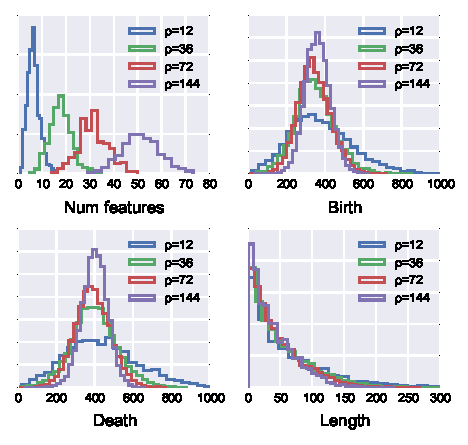
\includegraphics[width=\columnwidth]{./fig/coalescent_sims.pdf}}
\caption[Distributions of statistics defined on the $H_1$ persistence diagram for different model parameters]{Distributions of statistics defined on the $H_1$ persistence diagram for different model parameters. Top left: Number of features. Top right: Birth time distribution. Bottom left: Death time distribution. Bottom right: Feature length distribution. Data generated from $1000$ coalescent simulations with $n=100$, $\theta=500$, and variable $\rho$.}
\label{fig:coalescent_sims}
\end{center}
\end{figure}

\section{Statistical Model}
\label{sec:model}

The persistence diagram from a typical coalescent simulation is shown in Figure \ref{fig:persistence_diagram}.
Examining the diagram, it would be difficult to classify the observed features into signal and noise.
Instead, we use the information in the diagram to construct a statistical model in order to infer the parameters, $\theta$ and $\rho$, which generated the data.
Note that we consider inference using only $H_1$ invariants, but the ideas easily generalize to higher dimensions.
We consider the following properties of the persistence diagram: the total number of features, $K$; the set of birth times, $(b_1,{\ldots},b_K)$; the set of death times, $(d_1,{\ldots},d_K)$; and the set of persistence lengths, $(l_1,{\ldots},l_K)$.
In Figure \ref{fig:coalescent_sims} we show the distributions of these properties for four values of $\rho$, keeping fixed $n=100$ and $\theta=500$.
Several observations are immediately apparent.
First, the topological signal is remarkably stable.
Second, higher $\rho$ increases the number of features, consistent with the intuition that recombination generates nontrivial topology in the model.
Third, the mean values of the birth and death time distributions are only weakly dependent on $\rho$ and are slightly smaller than $\theta$, suggesting that $\theta$ defines a natural scale in the topological space.
However, higher $\rho$ tightens the variance of the distributions.
Finally, persistence lengths are independent of $\rho$.

Examining Figure \ref{fig:coalescent_sims}, we can postulate: $K \sim \mathrm{Pois}(\zeta)$, $b_k \sim \mathrm{Gamma}(\alpha,\xi)$, and $l_k \sim \mathrm{Exp}(\eta)$.
Death time is given by $d_k=b_k+l_k$, which is incomplete Gamma distributed.
The parameters of each distribution are assumed to be an \emph{a priori} unknown function of the model parameters, $\theta$ and $\rho$, and the sample size, $n$.
Keeping $n$ fixed, and assuming each element in the diagram is independent, we can define the full likelihood as
\begin{equation}
p(D \given \theta,\rho) = p(K \given \theta,\rho)\displaystyle\prod_{k=1}^{K}p(b_k \given \theta,\rho)p(l_k  \given \theta,\rho).
\end{equation}
Simulations over a range of parameter values suggest the following functional forms for the parameters of each distribution.
The number of features is Poisson distributed with expected value
\begin{equation}
\zeta=a_{0}\log\left(1+\frac{\rho}{a_{1}+a_{2}\rho}\right)
\end{equation}
Birth times are Gamma distributed with shape parameter
\begin{equation}
\alpha=b_{0}\rho+b_{1}
\end{equation}
and scale parameter
\begin{equation}
\xi = \frac{1}{\alpha}(c_{0}\exp(-c_{1}\rho)+c_{2}).
\end{equation}
These expressions appears to hold well in the regime $\rho<\theta$, but break down for large $\rho$.
The length distribution is exponentially distributed with shape parameter proportional to mutation rate, $\eta=\alpha\theta$.
The coefficients in each of these functions are calibrated using simulations, and could be improved with further analysis.
This model has a simple structure and standard maximum likelihood approaches can be used to find optimal values of $\theta$ and $\rho$.

\section{Experiments}
\label{sec:experiments}

\subsection{Coalescent Simulations}

We simulated a coalescent process with sample size $n=100$ and $l=10{,}000$ loci.
The mutation rate, $\theta$, was varied across $\theta=\{50,500,5000\}$.
The recombination rate, $\rho$, was varied across $\rho=\{4,12,36,72\}$.
The output of the process is a set of binary sequences of variable length (length is dependent on $\theta$).
The Hamming metric is used to construct a pairwise distance matrix between sequences.
We computed persistent homology and used the model described in Section \ref{sec:model} to estimate $\theta$ and $\rho$.
Results are shown in Figure \ref{fig:param_inference}, where we plot estimates and 95\% confidence interval from $500$ simulations.
We observe an improved $\rho$ estimate at higher mutation rate.
This is expected, as increasing $\theta$ is essentially increasing sampling on branches in the genealogy.
We also observe tighter confidence intervals at higher recombination rates, consistent with the behavior seen in Figure \ref{fig:coalescent_sims}.

\begin{figure}
\begin{center}
\centerline{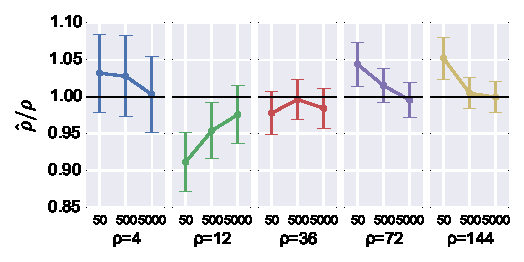
\includegraphics[width=\columnwidth]{./fig/param_inference.pdf}}
\caption{Inference of recombination rate $\rho$ using topological information. The recombination rate $\rho$ is estimated for five values \{4, 12, 36, 72, 144\} at three different mutation rates \{50, 500, 5000\}. Mean estimate over 500 simulations and 95\% confidence interval is shown.}
\label{fig:param_inference}
\end{center}
\end{figure}
\lipsum

\chapter{Reticulate Complex Constructions}
\label{ch:complex_construction}
\lipsum

%% Part 2: Microbes
\part{Applications: Microorganism Evolution}
\label{part:microorganism}

\chapter{Bacteriophage Reticulate Evolution}
\label{ch:phage}
\lipsum

\chapter{Influenza Evolution}
\label{ch:influenza}
%!TEX root = ../thesis.tex

In this chapter we analyze influenza.
Influenza is useful to examine because there is a lot of data.

\section{Influenza Virus}

Influenza is a single-stranded RNA virus that is naturally found in avian populations.
Each viral genome has eight genetic segments.

\section{Multiscale Flu Reassortment}

\begin{figure}
\begin{center}
\centerline{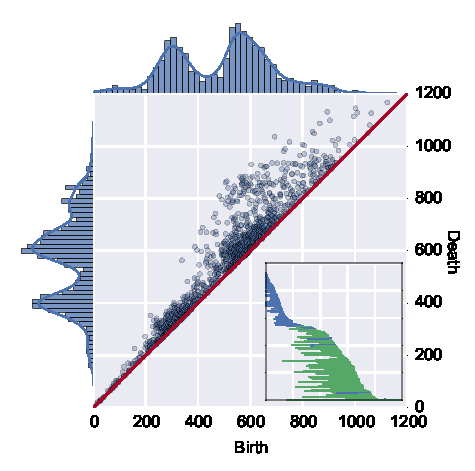
\includegraphics[width=\columnwidth]{./fig/flu_scatterplot.pdf}}
\label{fig:flu_scatterplot}
\caption[$H_1$ persistence diagram computed from an avian influenza dataset.]{The $H_1$ persistence diagram computed from an avian influenza dataset. On the top and left are plotted the marginal distributions of birth and death times, along with a density estimate for each distribution. The bimodality indicates two scales of topological structure. Inset: The barcode diagram for a subset of this data. Blue bars have representative cycles involving only one subtype, green bars have cycles involving multiple subtypes.}
\end{center}
\end{figure}

To test our model on biological data, we considered reassortment in avian influenza virus.
Influenza is a single-stranded RNA virus that is naturally found in avian populations.
Each viral genome has eight genetic segments.
Subtypes are defined by two segments, hemagglutinin (HA) and neuraminidase (NA), e.g. H1N1 and H3N2.
When a host cell is coinfected with two different viral strains, reassortment of these segments can occur, such that viral offspring is a genetic mixture of the two parental strains.
Reassortment is of substantial medical interest, and has been connected with the outbreak of influenza epidemics.

We computed persistent homology on an aligned dataset of 3,105 avian influenza sequences across the seven major HA subtypes.
The persistence diagram is shown in Figure \ref{fig:flu_scatterplot}, along with density estimates for the birth and death distributions.
Both birth and death times appear strongly bimodal, unlike in the coalescent simulations, which were strictly unimodal.
This suggests two distinct scales of topological structure.
Using the representative cycles output by Dionysus on a subset of this data, we classified features as intrasubtype (involving one HA subtype) and intersubtype (involving multiple HA subtypes).
The $H_1$ barcode diagram for this data is shown in the Figure \ref{fig:flu_scatterplot} inset.
Intrasubtype features, in blue, occur at an earlier filtration scale than intersubtype features, in green.
The multiscale topological approach of persistent homology can distinguish biological events occuring at different genetic scales.

We isolated the two peaks and estimated two recombination rates: an intrasubtype $\rho_{1}=9.68$, and an intersubtype $\rho_{2}=21.43$.
We conclude that intersubtype recombination occurs at a rate over twice that of intrasubtype recombination, however a genetic barrier exists that maintains distinct subtype populations.
The nature of this barrier warrants further study.
This illustrates a real world example in which multiscale topological structure can be captured by persistent homology and given biological interpretation.

\section{Prediction of Host Specific Residues}

In this section, we describe work in prediction of host specific residues using machine learning approaches.
Host specific residues are important for viral surveillance in order to predict possible outbreaks.
We describe here two methods and include preliminary validation from our collaborator in Wisconsin.

\chapter{Pathogen Evolution - PATRIC}
\label{ch:pathogens}
\lipsum

\chapter{Prokaryote Reticulate Evolution - COGs}
\label{ch:prokaryotes}
\lipsum
% %!TEX root = ../../thesis.tex
\chapter{Prokaryote Reticulate Evolution - Tree of Life}
\label{ch:prokaryotes}

In this chapter we examine evolutionary relationships across the prokaryotic domain.
As input data, we use the Cluster of Orthologous Genes (COG) database at NCBI \cite{Galperin:2014ua}.
Using a combination of topological tools, we present a construction meant to extend the tree of life paradigm.

\section{Introduction}

In this chapter, we examine evolutionary relationships across the prokaryotic domain.

First, we use persistent homology to characterize reticulation.
Second, we use mapper to visualize evolutionary relationships.

\section{Materials and Methods}

As input data, we use the Cluster of Orthologous Genes (COG) database from NCBI \cite{Galperin:2014ua}

\section{Results}

To visualize relationships, we use the Mapper algorithm, as implemented in Ayasdi Iris.

\section{Conclusion}

In this chapter, we have examined evolutionary relationships across the prokaryotic domain.


%% Part 3: Human Data
\part{Applications: Human Genomic Data}
\label{part:human}

\chapter{Human Recombination Rate Mapping}
\lipsum

\chapter{Human Population Structure}
\lipsum

\chapter{Human Chromsomal Organization}
\lipsum
% \input{./tex/human.tex}

\chapter{Conclusions}
\label{ch:conclusions}
\lipsum
% %!TEX root = ../thesis.tex
\chapter{Conclusions}

In this thesis we considered several problems in genomic and evolution.
Future work will continue in this direction.

\backmatter

\SingleSpacing
\printbibliography

\end{document}
